\documentclass[]{article}

\usepackage{amsfonts} 
\usepackage{amsmath}
\usepackage[margin=3cm]{geometry}
\usepackage{enumitem}
\usepackage{amsthm}
\usepackage{multirow}
\usepackage{listings}
\usepackage{xcolor}
\usepackage{graphicx}

\renewcommand*{\proofname}{Beweis}
\newenvironment{ausarbeitung}{\vspace{3mm}\noindent\textit{Ausarbeitung.}}{}

\definecolor{codegreen}{rgb}{0,0.6,0}
\definecolor{codegray}{rgb}{0.5,0.5,0.5}
\definecolor{codepurple}{rgb}{0.58,0,0.82}
\definecolor{backcolour}{rgb}{0.95,0.95,0.92}

\lstdefinestyle{mystyle}{
	backgroundcolor=\color{backcolour},   
	commentstyle=\color{codegreen},
	keywordstyle=\color{magenta},
	numberstyle=\tiny\color{codegray},
	stringstyle=\color{codepurple},
	basicstyle=\ttfamily\footnotesize,
	breakatwhitespace=false,         
	breaklines=true,                 
	captionpos=b,                    
	keepspaces=true,                 
	numbers=left,                    
	numbersep=5pt,                  
	showspaces=false,                
	showstringspaces=false,
	showtabs=false,                  
	tabsize=2
}

\lstset{style=mystyle}


%opening
\title{Abschlussprojekt}
\author{Ida Hönigmann \and Fabian Dopf}

\begin{document}

\maketitle

\section*{Aufgabe 1: Aufwandsordnung numerischer Verfahren}
Wir betrachten ein abstraktes numerisches Verfahren, das für $N \in \mathbb{N}$ Eingabedaten eine Laufzeit von $y_N \in \mathbb{R}_+$ hat. Man sagt, das Verfahren habe Aufwandsordnung $p > 0$, falls eine Konstante $C > 0$ existiert, sodass $y_N \leq C N^p$ für alle $N \in \mathbb{N}$.

\subsection*{Teilaufgabe 1a:}
Die Aufwandsordnung lässt sich über die Folge $\{p_N\}_{N \in \mathbb{N}}$ mit

\begin{align}
	\label{eq:def_N}
	p_N = \frac{\log(y_{2N})-\log(y_n)}{\log(2)} \text{ für } N \in \mathbb{N}
\end{align}

quantifizieren. Beachten Sie, dass die Bestimmung von $p_N$ die Verfügbarkeit von zwei aufeinanderfolgenden Folgengliedern $y_N$ und $y_{2N}$ erfordert. Verwenden Sie den Ansatz $y_N = CN^p$ und leiten Sie die Formel in \ref{eq:def_N} her!

\begin{proof}
	Annahme: $\forall N \in \mathbb{N}$ ist $p_N$, sodass $y_N \leq C N^{p_N}$ für ein $C > 0$.
	
	Für ein beliebiges $N \in \mathbb{N}$ gilt $\exists C_{1N}, C_{2N} > 0$ und $p_{1N}, p_{2N} > 0$ mit $y_N \leq C_{1N} N^{p_{1N}}$ und $y_{2N} \leq C_{2N} (2N)^{p_{2N}}$.
	
	Für $C:=max\{C_{1N}, C_{2N}\}$ und $p_N:=max\{p_{1N}, p_{2N}\}$ gilt $y_N \leq C_{1N} N^{p_{1N}} \leq C N^{p_N}$ und $y_{2N} \leq C_{2N} (2N)^{p_{2N}} \leq C (2N)^{p_N}$.
	 
	\begin{align}
		\log(y_{2N}) - \log(y_N) = \log\left(\frac{y_{2N}}{y_N}\right) = \log\left(\frac{C(2N)^{p_N}}{C\cdot N^{p_N}}\right) = \log(2^{p_N}) = p_N \log(2) \\
		\implies p_N = \frac{\log(y_{2N}) - \log(y_N)}{\log(2)}
	\end{align}

	TODO ob das so alles passt...

\end{proof}

\subsection*{Teilaufgabe 1b:}
Sei $\{\delta_N\}_{N \in \mathbb{N}} \subseteq \mathbb{R}$ eine Nullfolge, d.h. es gilt $\delta_N \rightarrow 0$ für $N \rightarrow \infty$. Weiters verhalte sich die Laufzeit wie $y_N = (C+\delta_N)N^p$ mit $C > 0$. Zeigen Sie, dass die Folge $\{p_N\}_{N \in \mathbb{N}}$ gegen $p$ konvergiert, d.h. es gilt $p_N \rightarrow p$ für $N \rightarrow \infty$.

\begin{proof}	
	Zuerst berechnen wir einen Grenzwert, den wir in späterer Folge verwenden werden. Die Gleichungen stimmen, da $\lim$ stetig ist und da laut Voraussetzung $\delta_N$ und somit auch $\delta_{2N}$ als Teilfolge, gegen $0$ konvergieren.
	
	\begin{align}
		\lim\limits_{n\rightarrow\infty} \log\left(\frac{C+\delta_{2N}}{C+\delta_N}\right) = \log\left(\lim\limits_{n\rightarrow\infty}\frac{C+\delta_{2N}}{C+\delta_N}\right) = \log\left(\frac{\lim\limits_{n\rightarrow\infty}C+\delta_{2N}}{\lim\limits_{n\rightarrow\infty}C+\delta_N}\right) = \log\left(\frac{C}{C}\right) = \log(1) = 0
	\end{align}

	Wir berechnen $\lim\limits_{n\rightarrow\infty}p_n$ indem wir die Gleichung \ref{eq:def_N} verwenden. Durch Einsetzen von $y_N = (C+\delta_N)N^p$ und den Rechenregeln von Limiten und dem Logarithmus erhalten wir folgendes:

	\begin{align}
		\implies
		p_N = \frac{\log(y_{2N}) - \log(y_N)}{\log(2)} = \frac{\log((C+\delta_{2N})(2N)^p) - \log((C+\delta_N)N^p)}{\log(2)} = \frac{\log\left(\frac{(C+\delta_{2N})(2N)^p}{(C+\delta_N)N^p}\right)}{\log(2)} \\
		= \frac{\log\left(\frac{(C+\delta_{2N})2^p}{(C+\delta_N)}\right)}{\log(2)} = \frac{p \log(2) + \log\left(\frac{C+\delta_{2N}}{C+\delta_N}\right)}{\log(2)} = p + \frac{\log\left(\frac{C+\delta_{2N}}{C+\delta_N}\right)}{\log(2)} \xrightarrow{n\rightarrow\infty} p + 0 = p
	\end{align}
	
	Zusammenfassend gilt nun $\lim\limits_{n\rightarrow\infty}p_n = p$, was zu zeigen war.

\end{proof}

\subsection*{Teilaufgabe 1c:}
In sogenannter doppelt logarithmischer Darstellung (log-log Plots) wird für beide Koordinatenachsen eine logarithmische Skalierung verwendet, d.h. sowohl die waagrechte als auch die senkrechte Koordinatenachse wird logarithmisch unterteilt. Wie werden Potenzfunktionen der Form $y = c x^p$ in einem log-log Plot dargestellt? Wie können Sie die Ordnung $p$ und die Konstante $c > 0$ aus einem log-log Plot von $y = cx^p$ direkt auslesen?

Darstellung ist Gerade. $c = f(1)$ und $p$ ist Steigung, wenn beide Achsen ''gleich'' skaliert.

\section*{Aufgabe 2: Cholesky-Verfahren und Skyline-Matrizen}
Eine Matrix $A \in \mathbb{R}^{n\times n}$ heißt Skyline-Matrix, falls es für $l = 1, ..., n$ Zahlen $p_l, q_l \in \mathbb{N}_0$ gibt, sodass für die $i$-te Zeile und $j$-te Spalte von $A$ gilt:

\begin{itemize}
	\item $A_{i,k} = 0 \text{ für } k < i - p_i$,
	\item $A_{k,j} = 0 \text{ für } k < j - q_j$,
\end{itemize}

Folgendes Beispiel illustriert diese Aussage:

\begin{align*}
	A = \begin{pmatrix}
		1 &   &   &   & 1 \\
		  & 1 &   & 2 & 2 \\
		  &   & 1 & 3 & 3 \\
		1 & 2 & 3 &14 &18 \\
		  & 4 & 5 &29 &48 \\
	\end{pmatrix}.
\end{align*}

\subsection*{Teilaufgabe 2a:}
Beweisen Sie, dass das Cholesky-Verfahren genau dann wohldefiniert ist (d.h. es wird nicht durch Null dividiert oder die Wurzel aus einer negativen Zahl gezogen), wenn die Matrix $A \in \mathbb{R}^{n\times n}$ symmetrisch und positiv definit ist.

\begin{proof}
	Wir wiederholen zuerst die relevanten Definitionen.
	
	Eine Matrix $A \in \mathbb{R}^{n\times n}$ heißt symmetrisch, falls $A = A^T$.
	
	Eine Matrix $A \in \mathbb{R}^{n\times n}$ heißt positiv definit, falls $\forall u \in \mathbb{R}^n\setminus\{0\}: u^T A u > 0$.
	
	Wir zeigen $\forall A \in \mathbb{K}^{n\times n}$ symmetrisch und positiv definit $\exists L \in \mathbb{R}^{n\times n}$ untere Dreiecksmatrix $: LL^T=A$ durch vollständige Induktion nach $n$.
	
	\begin{itemize}
		\item \textbf{Induktionsanfang:} $n=1$
		
		Wenn $A := \begin{pmatrix}
			a_{11}
		\end{pmatrix} \in \mathbb{R}^{1\times 1}$ eine beliebige symmetrische und positiv definite Matrix ist, folgt aus positiv definit, dass für
	
		\begin{align*}
			u := \begin{pmatrix}
				1
			\end{pmatrix} \in \mathbb{R}^1 \setminus\{0\} && 0 < u^TAu = \begin{pmatrix}
				1
			\end{pmatrix} \begin{pmatrix}
				a_{11}
			\end{pmatrix} \begin{pmatrix}
				1
			\end{pmatrix} = a_{11}
		\end{align*}
	
		Da also $a_{11} > 0$ gilt, ist $L := \begin{pmatrix}
			\sqrt{a_{11}}
		\end{pmatrix} \in \mathbb{R}^{1}$ wohldefiniert. Dann gilt
	
		\begin{align*}
			LL^T = \begin{pmatrix}
				\sqrt{a_{11}}
			\end{pmatrix} \begin{pmatrix}
				\sqrt{a_{11}}
			\end{pmatrix} = \begin{pmatrix}
				a_{11}
			\end{pmatrix} = A
		\end{align*}
	
		\item \textbf{Induktionsvoraussetzung:} $\forall A \in \mathbb{R}^{n \times n}$ symmetrisch und positiv definit $\exists L \in \mathbb{R}^{n\times n}$ untere Dreiecksmatrix $:LL^T=A$.
		
		\item \textbf{Induktionsschritt:} $n-1 \implies n$
		
		Sei $A \in \mathbb{R}^{n\times n}$ eine symmetrische und positiv definite Matrix. Wir definieren eine Matrix $B \in \mathbb{R}^{(n-1)\times(n-1)}$ durch $B_{i,j} := A_{i,j}$, einen Vektor $a \in \mathbb{R}^{n-1}$ durch $a_i := A_{i,n}$ und eine Zahl $\alpha \in \mathbb{R}$ durch $\alpha := A_{n,n}$.
		
		Zusammengefasst gilt nun
		
		\begin{align*}
			A = \begin{pmatrix}
				B & a \\
				a^T & \alpha
			\end{pmatrix} && \text{ wobei sich das }a^T\text{ aus der Symmetrie von }A\text{ ergibt.}
		\end{align*}
	
		Für $B$ gilt, dass es sich um eine symmetrische und positiv definite Matrix aus $\mathbb{R}^{(n-1)\times(n-1)}$ handelt. Laut Induktionsvoraussetzung existiert dazu eine untere Dreiecksmatrix $P \in \mathbb{R}^{(n-1)\times(n-1)}$ mit $PP^T=B$.
		
		Da $B$ positiv definit ist und somit regulär ist, folgt die eindeutige Existenz eines Vektors $l \in \mathbb{R}^{n-1}$ der die Gleichung $Pl=a$ erfüllt.
		
		Wir wollen nun $\beta \in \mathbb{R}$ so definieren, dass $\beta = \sqrt{\alpha - l^Tl}$. Dazu müssen wir sicherstellen, dass $\alpha - l^Tl > 0$.
		
		Wenn wir die Definition von $l$ verwenden und Umformen erhalten wir
		
		\begin{align*}
			\alpha - l^Tl &= \alpha - (P^{-1}a)^T(P^{-1}a) = \alpha - a^T (P^{-1})^TP^{-1}a \\
			&= \alpha - a^T (PP^T)^{-1}a = \alpha - a^T B^{-1}a
		\end{align*}
	
		Da $A$ positiv definit ist ergibt sich
	
		\begin{align*}
			0 < \begin{pmatrix}
				-B^{-1}a\\
				1
			\end{pmatrix}^T
			\underbrace{\begin{pmatrix}
				B & a\\
				a^T & \alpha
			\end{pmatrix}}_{=A}
			\begin{pmatrix}
				-B^{-1}a\\
				1
			\end{pmatrix} =
			\alpha - a^T B^{-1} a
		\end{align*}
	
		Also ist $\beta := \sqrt{\alpha - l^Tl}$ wohldefiniert. Umgeformt gilt nun $l^Tl + \beta^2 = \alpha$.
		
		Definieren wir nun $L \in \mathbb{R}^{n\times n}$ durch
		
		\begin{align*}
			L = \begin{pmatrix}
				P & 0 \\
				l^T & \beta
			\end{pmatrix}
		\end{align*}
	
		Dann gilt
		
		\begin{align*}
			LL^T = \begin{pmatrix}
				P & 0 \\
				l^T & \beta
			\end{pmatrix} \begin{pmatrix}
				P^T & l \\
				0 & \beta
			\end{pmatrix} = \begin{pmatrix}
				PP^T & Pl \\
				l^TP^T & l^Tl+\beta^2
			\end{pmatrix} = \begin{pmatrix}
				PP^T & Pl \\
				(Pl)^T & l^Tl+\beta^2
			\end{pmatrix} = \begin{pmatrix}
				B & a \\
				a^T & \alpha
			\end{pmatrix} = A
		\end{align*}
	\end{itemize}
	
\end{proof}

\subsection*{Teilaufgabe 2b:}
Beweisen Sie, dass die Besetzungsstruktur der Cholesky-Zerlegung der Skyline-Matrix $A$ erhalten bleibt, d.h. dass auch die untere Dreiecksmatrix $L$ eine geeignete Bandstruktur aufweist.

\begin{proof}
	TODO Beweis 2b
\end{proof}

\section*{Aufgabe 3: Pseudocode für Cholesky-Zerlegung von Skyline-Matrizen}
Verwenden Sie den Cholesky-Algorithmus aus der Vorlesung. Entwerfen Sie jeweils einen Pseudocode, der für eine Skyline-Matrix:
\subsection{Teilaufgabe 3a:}
möglichst effizient die Struktur erkennt.

\begin{lstlisting}[language=Python, caption=Strukturerkennung einer Skyline-Matrix]
	def to_skyline(matrix):
		values = list()
		
		for i in range(dim(matrix)):
		    up_branch = matrix[:, i][:i + 1]
		    up_branch.reverse()
		    while not up_branch.empty and up_branch[-1] == 0:
		        up_branch.pop(-1)
		
		    left_branch = matrix[i, :][:i]
		    left_branch.reverse()
		    while not left_branch.empty and left_branch[-1] == 0:
		        left_branch.pop(-1)
		
		    values.append([up_branch, left_branch])
		    
		return values
\end{lstlisting}

\begin{lstlisting}[language=Python, caption=Strukturerkennung einer symmetrischen positiv definiten Skyline-Matrix]
	def to_spd_skyline(matrix):
	    values = list()
	
	    for i in range(dim(matrix)):
	        branch = matrix[:, i][:i + 1]
	        branch.reverse()
	        while not branch.empty and branch[-1] == 0:
	            branch.pop(-1)
	
	        values.append(branch)
	        
	    return values
\end{lstlisting}

\subsection*{Teilaufgabe 3b:}
die Cholesky-Zerlegung berechnet.

\begin{lstlisting}[language=Python, caption=Algorithmus für die Cholesky Zerlegung einer Matrix]
	def cholesky(matrix):	
	    n = dim(matrix)
	    l = zero matrix of dimension n by n
	
	    for k in range(n):
	        s = 0
	        for j in range(k):
	            s += l[k, j] * l[k, j]
	
	        l[k, k] = sqrt(matrix[k, k] - s)
	
	        for i in range(k+1, n):
	            s = 0
	            for j in range(k):
	                s += l[i, j] * l[k, j]
	                
	            l[i, k] = (matrix[i, k] - s) / l[k, k]
	
	    return l
\end{lstlisting}

\begin{lstlisting}[language=Python, caption=optimierter Algorithmus für die Cholesky Zerlegung einer Skyline-Matrix]
	def cholesky_skyline(values):
	    n = len(values)
	    l = zero matrix of dimension n by n
	
	    max_width = max(len(branch) for branch in values)
	
	    for k in range(n):
	        start_idx = k - len(values[k]) + 1
	        s = np.dot(l[k][start_idx:k], l[k][start_idx:k])
	        l[k, k] = sqrt(self[k, k] - s)
	
	        for i in range(k + 1, min(k + max_width, n)):
	            if k > i - len(values[i]):
	                s = np.dot(l[i][start_idx:k], l[k][start_idx:k])
	                l[i, k] = (self[i, k] - s) / l[k, k]
	
	    return l
\end{lstlisting}

\section*{Aufgabe 4: Aufwand des Algorithmus und Verhalten in Spezialfällen}
\subsection*{Teilaufgabe 4a:}
Sei $A \in \mathbb{R}^{n\times n}$ eine Skyline-Matrix. Welchen Aufwand haben Ihre Algorithmen aus Aufgabe 3 in Abhängigkeit von der Größe $n$ der Eingabedaten und Skyline-Indices $p_l = q_l$?

\begin{ausarbeitung}
	
	\begin{itemize}
		\item \texttt{to\_skyline} hat wegen den Schleifen in Zeile 4, 7 und 12 Aufwand $\sum_{l=1}^{n} (n-p_l)+(n-q_l) = 2n^2-\sum_{l=1}^{n}p_l+q_l$.
		\begin{itemize}
			\item best case: Im besten Fall sind $p_l = l$ und $q_l = l$ also maximal, was zu einem Aufwand von $2n^2-\sum_{l=1}^{n}2l = 2n^2 - 2\frac{n(n+1)}{2} = 2n^2-(n^2+n) = n^2 - n$ führt
			\item worst case: Im schlechtesten Fall sind $p_l=0$ und $q_l = 0$ also minimal, was in zu einem Aufwand von $2n^2 - \sum_{l=1}^{n}0 = 2n^2$ führt
		\end{itemize}
		
		\item \texttt{to\_spd\_skyline} hat wegen den Schleifen in Zeile 4 und 7 Aufwand $\sum_{l=1}^{n}(n-p_l) = n^2 - \sum_{l=1}^{n}p_l$
		\begin{itemize}
			\item best case: Im besten Fall ist $p_l = l$ also maximal, was zu einem Aufwand von $n^2 - \sum_{l=1}^{n}l = n^2 - \frac{n(n+1)}{2} = n^2 - \frac{1}{2}n^2 - \frac{1}{2}n = \frac{1}{2}(n^2-n)$ führt
			\item worst case: Im schlechtesten Fall ist $p_l=1$ also minimal, was in zu einem Aufwand von $n^2 - \sum_{l=1}^{n}1 = n^2 - n$ führt
		\end{itemize}
	
		\item \texttt{cholesky} hat wegen den Schleifen in Zeile 5, 7, 12 und 14 Aufwand $\sum_{k=1}^{n}(k + \sum_{i=k+1}^{n}k) = \sum_{k=1}^{n}(k+k(n-k)) = \sum_{k=1}^{n}k + \sum_{k=1}^{n}kn - \sum_{k=1}^{n}k^2 = \frac{n(n+1)}{2} + \frac{n^2(n+1)}{2} - \frac{n(n+1)(2n+1)}{6} = \frac{1}{6}n^3 + \frac{1}{2}n^2 + \frac{1}{3}n$ also $\mathcal{O}(n^3)$
		
		\item \texttt{cholesky\_skyline} Zeilen 9 und 14 haben Aufwand $\mathcal{O}(p_k)$, da die beiden Vektoren Länge $k - start\_idx + 1 = k - (k - p_k + 1) + 1 = p_k$ haben und sind somit, neben Zeile 5 mit Aufwand von $\mathcal{O}(n)$, die aufwändigsten Zeilen in der Funktion.
		
		Durch das if-Statement in Zeile 13 wird sichergestellt, dass der Aufwand nur anfällt, falls nach Aufgabe 2b das Ergebnis nicht trivial ist.
		
		Die Einschränkung in Zeile 12 auf den Bereich \texttt{range(k+1, k+max\_width)} statt \texttt{range(k+1, n)} ermöglicht es viele der if-Statements zu ersparen, die es dem Python-Interpreter erschweren die Ausführung zu optimieren\footnote{If-Statements ermöglichen es nicht die Instruction Pipeline vollständig auszunützen und verlangsamen dadurch die Ausführung. In modernen Systemen wird daher sogenannte Branch Prediction durchgeführt die versucht vorherzusagen ob die Bedingung wahr ist.}.
		
		Insgesamt ist der Aufwand also $n + \sum_{k=1}^{n} \sum_{l=1}^{p_k}p_k = n + \sum_{k=1}^{n} p_k^2$ was  
		\begin{itemize}
			\item im besten Fall $n + \sum_{k=1}^{n} 1 = 2n$ und
			\item im schlechtesten Fall $n + \sum_{k=1}^{n}k^2 = n + \frac{n(n+1)(2n+1)}{6} = \frac{1}{3}n^3 + \frac{1}{2}n^2 + \frac{7}{6}n$ ist.
		\end{itemize}
	\end{itemize}
	
\end{ausarbeitung}


\subsection*{Teilaufgabe 4b:}
Betrachten Sie Matrizen mit den Besetzungsstrukturen

\begin{align*}
	\begin{pmatrix}
		* & * & * & * & *\\
		* & * &   &   &  \\
		* &   & * &   &  \\
		* &   &   & * &  \\
		* &   &   &   & *\\
	\end{pmatrix}
	\text{ bzw. }
	\begin{pmatrix}
	* &   &   &   & *\\
	  & * &   &   & *\\
	  &   & * &   & *\\
	  &   &   & * & *\\
	* & * & * & * & *\\
\end{pmatrix}
\end{align*}

Welche Besetzungsstruktur hat die Cholesky-Zerlegung für beide Matrizen? Was könnte man machen, um für Matrizen mit der ''linken'' Besetzungsstruktur die Cholesky-Zerlegung effizienter zu berechnen?

\begin{ausarbeitung}
	Die linke Matrix ist vollbesetzt als Skyline-Matrix, in dem Sinne, dass $\forall k \in \{1, ..., n\}: p_k = q_k = k$ also immer den maximal möglichen Wert annimmt.
	
	Die rechte Matrix hat die Skyline-Indizes $\forall k \in \{1, ..., n - 1\}: p_k = q_k = 1$ und $p_n = q_n = n$ und ist daher nach Aufgabe 4a effizienter in der Berechnung der Cholesky-Zerlegung.
	
	Eine effiziente Berechnung der Cholesky-Zerlegung der linken Matrix erhält man mit folgender Überlegung:
	
	Definieren wir eine Abbildung $\sigma: \mathbb{R}^{n\times n} \rightarrow \mathbb{R}^{n \times n}$ die einer Matrix $A$ die ''gespiegelte'' Matrix $\sigma(A)$ zuordnet wobei $(\sigma(A))_{i,j} := A_{n+1-j, n+1-i}$.
	
	$\sigma$ hat folgende Eigenschaften: Für beliebige $A,B \in \mathbb{R}^{n \times n}$ gilt
	
	\begin{itemize}
		\item Die Umkehrabbildung $\sigma^{-1} = \sigma$, da
			\begin{align*}
				\sigma(\sigma(A))_{ij} = \sigma(A)_{n+1-j,n+1-i} = A_{n+1-(n+1-i),n+1-(n+1-j)} = A_{i,j}
			\end{align*}
		
		\item Verträglich mit Transponieren
			\begin{align*}
				\sigma(A^T)_{i,j} = A^T_{n+1-j,n+1-i} = A_{n+1-i,n+1-j} = \sigma(A)_{j,i} = \sigma(A)^T_{i,j}
			\end{align*}
		\item Verträglich mit Multiplizieren
			\begin{align*}
				(\sigma(A)\sigma(B))_{i,j} &= \sum_{k=1}^{n}\sigma(A)_{i,k}\sigma(B)_{k,j} = \sum_{k=1}^{n} A_{n+1-k,n+1-i}B_{n+1-j,n+1-k} \\
				&= \sum_{k=1}^{n} B_{n+1-j,k}A_{k,n+1-i} = (BA)_{n+1-j,n+1-i} = \sigma(BA)_{i,j}
			\end{align*}
		
			da $k \mapsto n+1-k$ eine Permutation von $\{1, .., n\}$ ist.
		\item Dreiecksmatrix bleibt erhalten
		
		Wenn $A$ eine untere Dreiecksmatrix ist, also $A_{i,j} = 0$ für $i < j$, so folgt, dass $\sigma(A)$ auch eine untere Dreiecksmatrix ist, da $i < j \iff n+1-j < n+1-i$.
		
		\item Symmetrie bleibt erhalten
		
		Wenn $A$ symmetrisch ist, so ist auch $\sigma(A)$ symmetrisch, da $\sigma(A)_{i,j} = A_{n+1-j,n+1-i} = A_{n+1-i,n+1-j} = \sigma(A)_{j,i}$.	
	\end{itemize}

	Sei $A$ eine Matrix von der linken, ungünstigen Art. Dann ist $\sigma(A)$ von der rechten Art, und ist es ist daher möglich die Cholesky-Zerlegung von $\sigma(A)$ effizient zu berechnen. Sei $L$ eben diese Zerlegung von $\sigma(A)$, d.h. $LL^T=\sigma(A)$.
	
	Nach dem oben gezeigten gilt nun $\sigma(L)^T\sigma(L) = \sigma(L^T)\sigma(L) = \sigma(LL^T) = \sigma(\sigma(A)) = A$. Womit wir eine Cholesky-Zerlegung von $A$ erhalten.
\end{ausarbeitung}


\section*{Aufgabe 5: Implementierung des Algorithmus und empirische Aufwandsschätzung}
Implementieren Sie Ihren modifizierten Cholesky-Algorithmus in Python und weisen Sie empirisch nach, dass der Aufwand linear in $n$ wächst. Vergleichen Sie die Performance Ihrer Implementierung mit der Python-Funktion \texttt{scipy.linalg.cholesky}, wobei die Skyline-Matrix $A$ als vollbesetzte Matrix gespeichert ist.

\begin{ausarbeitung}
	TODO Anhang Python-Code (+ Grafik Performance?)
	
	\begin{figure}
		\centering
		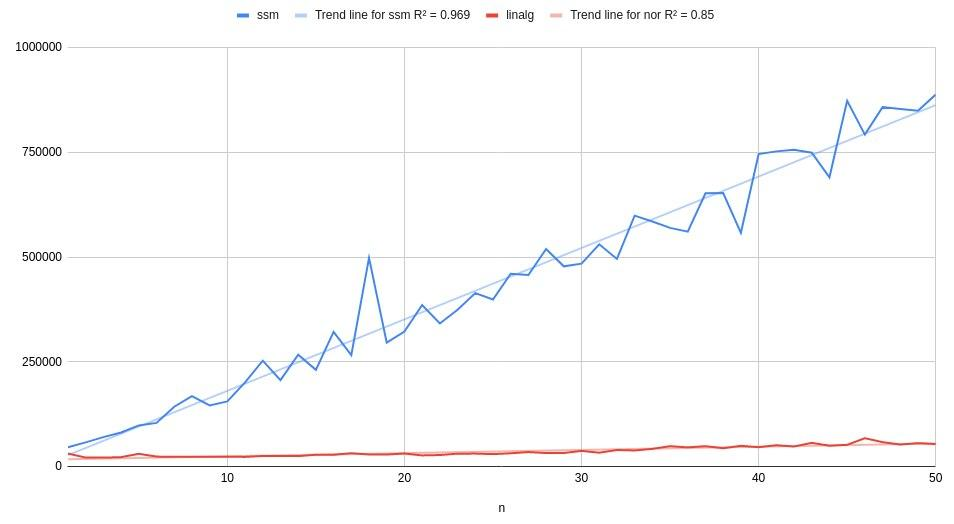
\includegraphics[width=\linewidth]{aufwand_cholesky}
		\caption{Aufwand \texttt{cholesky\_skyline} in blau und \texttt{linalg.choleksy} in rot; beides mit einer linearen Trendlinie}
		\label{fig:aufwandcholesky}
	\end{figure}
	
\end{ausarbeitung}

\end{document}
